% !TEX TS-program = pdflatex
% !TEX encoding = UTF-8 Unicode
% This is a simple template for a LaTeX document using the "article" class.
% See "book", "report", "letter" for other types of document.
\documentclass[14pt]{report} % use larger type; default would be 10pt
\usepackage[utf8]{inputenc} % set input encoding (not needed with XeLaTeX)

%%% Examples of Article customizations
% These packages are optional, depending whether you want the features they provide.
% See the LaTeX Companion or other references for full information.

%%% PAGE DIMENSIONS
\usepackage{geometry} % to change the page dimensions
\geometry{a4paper} % or letterpaper (US) or a5paper or....
% \geometry{margin=2in} % for example, change the margins to 2 inches all round
% \geometry{landscape} % set up the page for landscape
%   read geometry.pdf for detailed page layout information

\usepackage{graphicx} % support the \includegraphics command and options
\usepackage{float}
% \usepackage[parfill]{parskip} % Activate to begin paragraphs with an empty line rather than an indent

%%% PACKAGES
\usepackage{booktabs} % for much better looking tables
\usepackage{array} % for better arrays (eg matrices) in maths
\usepackage{paralist} % very flexible & customisable lists (eg. enumerate/itemize, etc.)
\usepackage{verbatim} % adds environment for commenting out blocks of text & for better verbatim
\usepackage{subfig} % make it possible to include more than one captioned figure/table in a single float
% These packages are all incorporated in the memoir class to one degree or another...

%%% HEADERS & FOOTERS
\usepackage{fancyhdr} % This should be set AFTER setting up the page geometry
\usepackage{lastpage}
\pagestyle{fancy} % options: empty , plain , fancy
\renewcommand{\headrulewidth}{1pt} % customise the layout...
\renewcommand{\footrulewidth}{0.7pt}
\lhead{}\chead{}\rhead[bfseries]{Melanoma Recognition Code Manual}
\lfoot{}\cfoot{Page \thepage\ of \pageref{LastPage}}\rfoot{}
%\usepackage{indentfirst}

%%% SECTION TITLE APPEARANCE
\usepackage{sectsty}

\allsectionsfont{\sffamily\mdseries\upshape} % (See the fntguide.pdf for font help)
% (This matches ConTeXt defaults)

%%% ToC (table of contents) APPEARANCE
\usepackage[nottoc,notlof,notlot]{tocbibind} % Put the bibliography in the ToC
\usepackage[titles,subfigure]{tocloft} % Alter the style of the Table of Contents
\renewcommand{\cftsecfont}{\rmfamily\mdseries\upshape}
\renewcommand{\cftsecpagefont}{\rmfamily\mdseries\upshape} % No bold!
\usepackage{xcolor}
\definecolor{mylink}{RGB}{3,54,73}
\definecolor{mylink2}{RGB}{3,101,100}
\usepackage[colorlinks, linkcolor=mylink2,anchorcolor=black,citecolor=green]{hyperref}
% load package with ``framed'' and ``numbered'' option.
\usepackage[framed,numbered,autolinebreaks,useliterate]{mcode}
\usepackage{cleveref}
%%% END Article customizations

%%% The "real" document content comes below...

\title{Melanoma Recognition Code Manual}
\author{Jiexin Guo, Junjian Xie \\ID:	14213839,	14213834}
\date{2014.11.29}

%\date{} % Activate to display a given date or no date (if empty),
         % otherwise the current date is printed 
\setcounter{tocdepth}{2}
\begin{document}

\maketitle
\clearpage

\tableofcontents
\clearpage

\chapter{Overview}
\clearpage
\section{Introduction}
	Melanoma is a type of skin cancer which forms from melanocytes (pigment-containing cells in the skin) and it is one kind of the skin cancer. 
	\begin{figure}[H]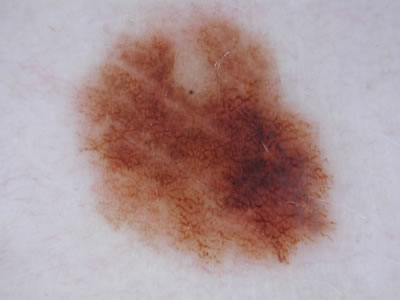
\includegraphics[width=\textwidth]{../dataset/cancer/pic_006.jpg} \caption{Melanoma}  \label{fig:introCancerImg} \end{figure}
	If melanoma is found early, while it is still small and thin, and if it is completely removed, then the chance of cure is high.However, it is much more dangerous if it is not found in the early stages. It causes the majority (75\%) of deaths related to skin cancer.
	So we try to find a way of image recognition to identify this disease and try to help.
	\\ \textbf{In the following passage we will use Melanoma or cancer refers to Melanoma.}
\section{Goal}
	Our goal is to develop a tool that can automatically recognize whether an image is of Melanoma , and its correct rate should be more than 80\%.
\section{Environment}
	Our program is developed using Matlab 2014a, with 64bit windows. Since we have used the Neural Network Toolbox to set up and train our neural network, you should run this code with a Matlab version(maybe 2009 or higher) that has the Neural Network Toolbox(nntool).
\section{Execution}
	Unzip the source file, do not change the directory structure, and you should see this:
	\begin{figure}[H]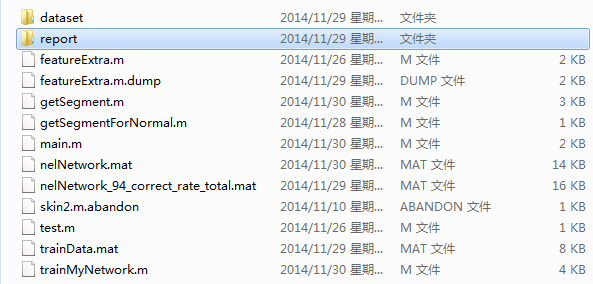
\includegraphics[width=\textwidth]{image/directory_structure.jpg} \caption{Directory structure}  \label{fig:dirStruct} \end{figure}
	Then open your Matlab and change the directory to this so that you can directly run the main.m . Next we will talk about every file's function in chapter 2.

\chapter{Code View}
\clearpage
\section{main.m}
\subsection{Function}
	This is the main entrance of the program.
\subsection{Accelerating the program}
	Please see this part in the section of \hyperref[subsection:Accelerating the program]{Accelerating the program} in the \hyperref[section:trainMyNetwork.m]{trainMyNetwork.m} section and also \hyperref[subsection:Accelerating the program2]{Accelerating the program} in the \hyperref[section:getSegment.m]{getSegment.m}.
\subsection{Parameters}
	The parameters are set in this .m file's line 4 to line 7, like below:
	\lstinputlisting[firstline=4, lastline=7]{../main.m}
\subsubsection{numberofCancer}
	This is the total number of cancer image, usually it should be equal to or less than the number of jpg files in \verb|dataset/cancer/|.
	\label{par:numberofCancer} 
\subsubsection{numberofOther}
	This is the total number of not cancer image(the opposite of our recognition,maybe normal skin or other skin disease), usually it should be equal to or less than the number of jpg files in \verb|dataset/normal/|.
	\label{par:numberofOther} 
\subsubsection{reComputeFeature}
	A boolean, if it is true, the program will recompute all the features of the first 'numberofCancer' files in \verb|dataset/cancer/| and all the first 'numberofOther' files in \verb|dataset/normal/|.\\
	For example, if reComputeFeature is true, numberofCancer is 56 and numberofOther is 32, then the program will compute the feature of the first 56 jpgs in \verb|dataset/cancer/| and first 32 jpgs in \verb|dataset/normal/| and save them into a file:'trainData.mat'.
	\\If it is set to be false, then the program will not recompute the feature but to load the features from file:'trainData.mat'.
	\label{par:reComputeFeature} 
\subsubsection{reTrainNetwork}
	Also a boolean.True tells the function 'trainMyNetwork' to retrain the network.	False will not retrain the network but to load the network from file: 'nelNetwork.mat'.
	\label{par:reTrainNetwork} 
\subsection{Output}
	\begin{figure}[H]
		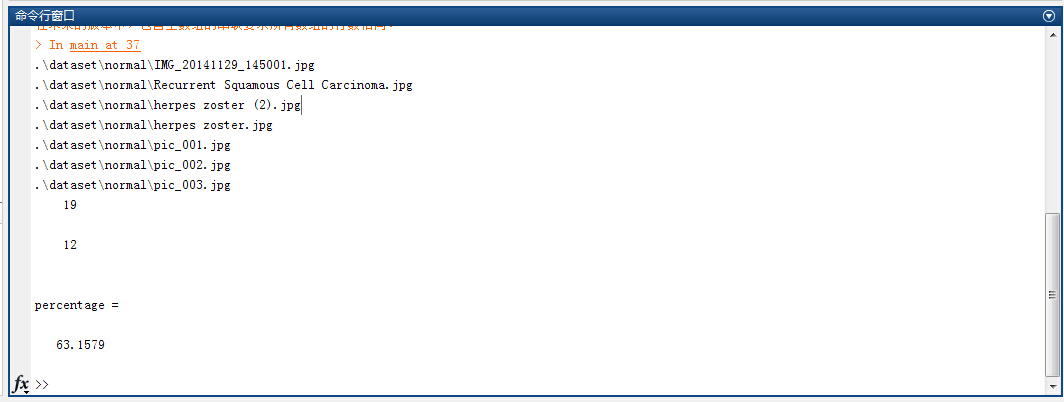
\includegraphics[width=\textwidth]{image/resultoftest.jpg} 
		\caption{Output of main.m} 
		 \label{fig:Outputofmain} 
	\end{figure}
	This is the console output of running main.m.
	\\The first several lines of file path are those recognition failed files' path.
	\\The next number 19 is the total test case number.
	\\The next number 12 is the test case number of correct recognition.
	\\The last number is the correct rate.
	\\Here is another example of our best correct rate using \verb|'nelNetwork_94_correct_rate_total.mat'| (please change this mat file's name to nelNetwork.mat and run):
	\begin{figure}[H]
		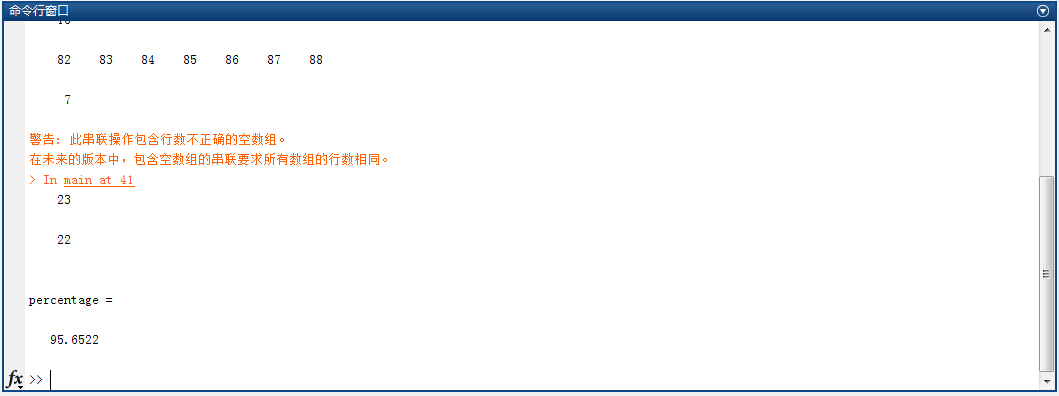
\includegraphics[width=\textwidth]{image/resultoftestbest.jpg} 
		\caption{Our best output of main.m} 
		 \label{fig:Outputbest} 
	\end{figure}
\subsection{Code of main.m}
\lstinputlisting{../main.m}

\clearpage
\section{trainMyNetwork.m}
\label{section:trainMyNetwork.m}
\subsection{Function}
	This .m file can recompute all the image files' feature (by calling getSegment.m) and set up and retrain the Neural Network(using some of the images as the trainning data set).
\subsection{Accelerating the program}
\label{subsection:Accelerating the program}
	The computation of feature may cost a lot of time, you can accelerate this procedure if you have a multiprocessor computer.
	\\You can change the code in this file at line 23 and 39(please open the matlabpool first:	\mcode{matlabpool open 8;}):
	\\\mcode{for i=1:numberofCancer}
	\\\mcode{for i=1:numberofOther}
	\\change these above two into:
	\\\mcode{parfor i=1:numberofCancer}
	\\\mcode{parfor i=1:numberofOther}
	\\Then you can use all the cpu to compute the features of image.But please ensure that your cpu will not get overheat.
\subsection{Input parameters}
\subsubsection{numberofCancer}
	It is the same as the parameter \hyperref[par:numberofCancer]{numberofCancer} in main.m.
\subsubsection{numberofOther}
	It is the same as the parameter \hyperref[par:numberofOther]{numberofOther} in main.m.
\subsubsection{retrainFea}
	A boolean the same as the parameter  \hyperref[par:reComputeFeature]{reComputeFeature}  in main.m.
\subsubsection{retrainNetwork}
	A boolean the same as the parameter  \hyperref[par:reTrainNetwork]{reTrainNetwork}  in main.m.
\subsection{Internal parameters}
	There are also some parameters can be set in this file,in line 7 to line 8:
	\lstinputlisting[firstline=7, lastline=8]{../trainMyNetwork.m}
	and also line 74 to line 76(network training parameter):
	\lstinputlisting[firstline=74, lastline=76]{../trainMyNetwork.m}
\subsubsection{trainNumberOfCancer}
	Using the first 1 to trainNumberOfCancer of the cancer images' features to train the network.
	\label{par:trainNumberOfCancer} 
\subsubsection{trainNumberOfOther}
	Using the first 1 to  trainNumberOfOther of the none cancer images' features to train the network.
	\label{par:trainNumberOfOther} 
\subsubsection{myNet.trainParam.lr}
	This defines the Neural Network's learning rate. If the rate is large, the training speed may increase but the network maybe hard to converge. If the rate is small, the speed of training will be slow but the network would be converged and stable.
	\\We set it to a default value 0.05.
\subsubsection{myNet.trainParam.goal}
	This is the target error of neural network training. Its default value is 0.01.
\subsubsection{myNet.trainParam.epochsl}
	This is the maximum value of training iteration. Default value is 10000.
\subsection{Output parameters}
\subsubsection{myNet}
	Returns the Neural Network.
\subsubsection{trainNumberOfCancer}
	The same as  \hyperref[par:trainNumberOfCancer]{trainNumberOfCancer}.
\subsubsection{trainNumberOfOther}
	The same as  \hyperref[par:trainNumberOfOther]{trainNumberOfOther}.
\clearpage
\subsection{Code of trainMyNetwork.m}
\lstinputlisting{../trainMyNetwork.m}

\clearpage
\section{getSegment.m}
\label{section:getSegment.m}
\subsection{Function}
	Use median filter to filter the image first. Then we use the active contour without edges algorithm to get the lesion area curve. After these, this function will set the area out of the curve to be blank and return this image.
\subsection{Accelerating the program}
\label{subsection:Accelerating the program2}
	The computation of feature may cost a lot of time, you can accelerate this procedure by decreasing the iteration time of this file in line 39:
	\lstinputlisting[firstline=39, lastline=39]{../getSegment.m}
	You can change the 700 to a smaller value, it can reduce  the time but may also reduce the correct rate.
\subsection{Input parameters}
\subsubsection{imgFilename}
	The path of the image.
\subsubsection{printImage}
	True if the user want to see the segment result. 
\subsection{Output parameters}
\subsubsection{X}
	Returns the image after segmentation.
\subsection{Output}
	If you set printImage=true, then you will see the next picture:
	\begin{figure}[H]
		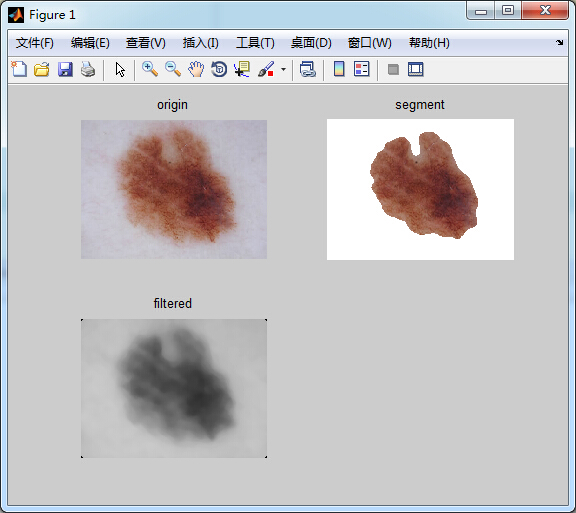
\includegraphics[width=\textwidth]{image/segmentResult.jpg} 
		\caption{getSegment.m output picture} 
		 \label{fig:OutputofgetSegment} 
	\end{figure}
	The image on the top left is the origin image. The one on the bottom left is the filtered image. And the last one is the segment result.
\clearpage
\subsection{Code of getSegment.m}
\lstinputlisting{../getSegment.m}

\clearpage
\section{featureExtra.m}
\subsection{Function}
Compute the feature vector of an image.Using 9 color features(3 for each color planes R G B) and 4 texture features.
\subsection{Input parameters}
\subsubsection{inputImage}
The RGB image matrix after median filtered and segmented.
\subsection{Output}
\subsubsection{outputX}
Returns a 13×1 feature vector.
	\begin{figure}[H]
		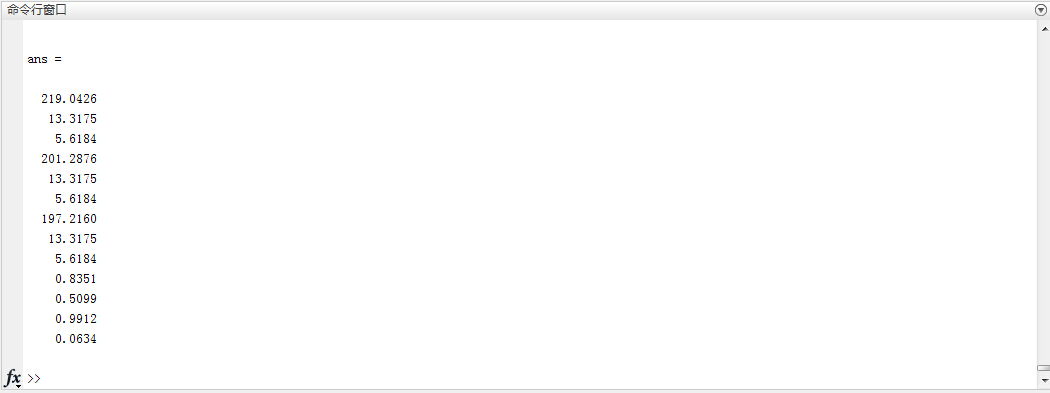
\includegraphics[width=\textwidth]{image/features.jpg} 
		\caption{Features} 
		 \label{fig:features} 
	\end{figure}
\clearpage
\subsection{Code of featureExtra.m}
\lstinputlisting{../featureExtra.m}
	
\chapter{Application}
\clearpage
\section{Image pipeline}
\subsection{Median filter}
	We first use the median filter to reduce the effect of noise or hear on the feature extraction(see  \hyperref[section:getSegment.m]{getSegment.m}). 
\subsection{Segmentation with Active contour without edges}
	Then we use the active contour without edges algorithm to segment the image and set the outter area of normal skin(we assume that the lesion area should be in the middle orof the image ) to be blank so that it won't have the effect on the feature extraction.
	\\And the result is like (or see  \hyperref[section:getSegment.m]{getSegment.m}):
	\begin{figure}[H]
		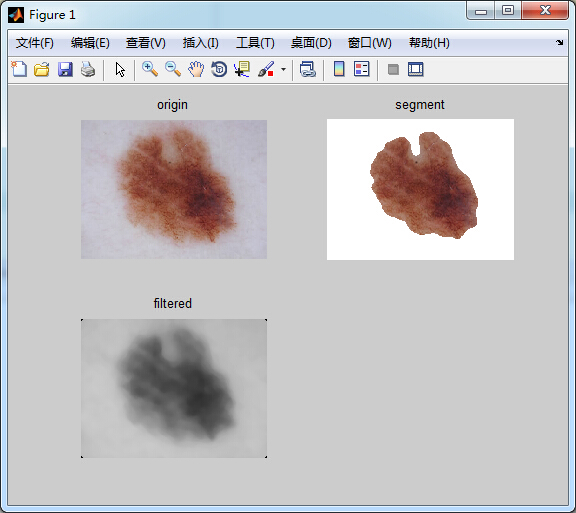
\includegraphics[width=\textwidth]{image/segmentResult.jpg} 
		\caption{getSegment.m output picture} 
		 \label{fig:OutputofgetSegment_copy1} 
	\end{figure}
\subsection{Feature extracion}
We use the three color moments \cref{eq:muc} \cref{eq:sigmac} \cref{eq:thetac} for each color plane(R G B),and form the first 9 feature:
\begin{equation}
\mu_{c} = \frac{1}{MN} \sum_{i=1}^M \sum_{j=1}^N p_{ij}^c
\label{eq:muc}
\end{equation}
\begin{equation}
\sigma_{c} = \left[\frac{1}{MN} \sum_{i=1}^M \sum_{j=1}^N \left(p_{ij}^c-\mu_{c}\right)^2 \right]^{1/2}
\label{eq:sigmac}
\end{equation}
\begin{equation}
\theta_{c} = \left[\frac{1}{MN} \sum_{i=1}^M \sum_{j=1}^N \left(p_{ij}^c-\mu_{c}\right)^3 \right]^{1/3}
\label{eq:thetac}
\end{equation}
Then we use another 4 features \cref{eq:Entropy} \cref{eq:Energy} \cref{eq:Contrast}  \cref{eq:Homogeneity} associated with gray level co-occurrence matrix C(i,j) :
\begin{equation}
Entropy = \sum_{i}\sum_{j}C\left(i,j\right)\log(C\left(i,j\right))
\label{eq:Entropy}
\end{equation}
\begin{equation}
Energy = \sum_{i}\sum_{j}C^2\left(i,j\right)
\label{eq:Energy}
\end{equation}
\begin{equation}
Contrast = \sum_{i}\sum_{j}\left(i-j\right)^2 C\left(i,j\right)
\label{eq:Contrast}
\end{equation}
\begin{equation}
Homogeneity = \sum_{i}\sum_{j}\frac{C\left(i,j\right)}{1+\left|i-j\right|}
\label{eq:Homogeneity}
\end{equation}
\section{Dataset}
	We divide the total dataset into two classes : the Melanoma class and the none Melanoma class. 
	\begin{figure}[H]
		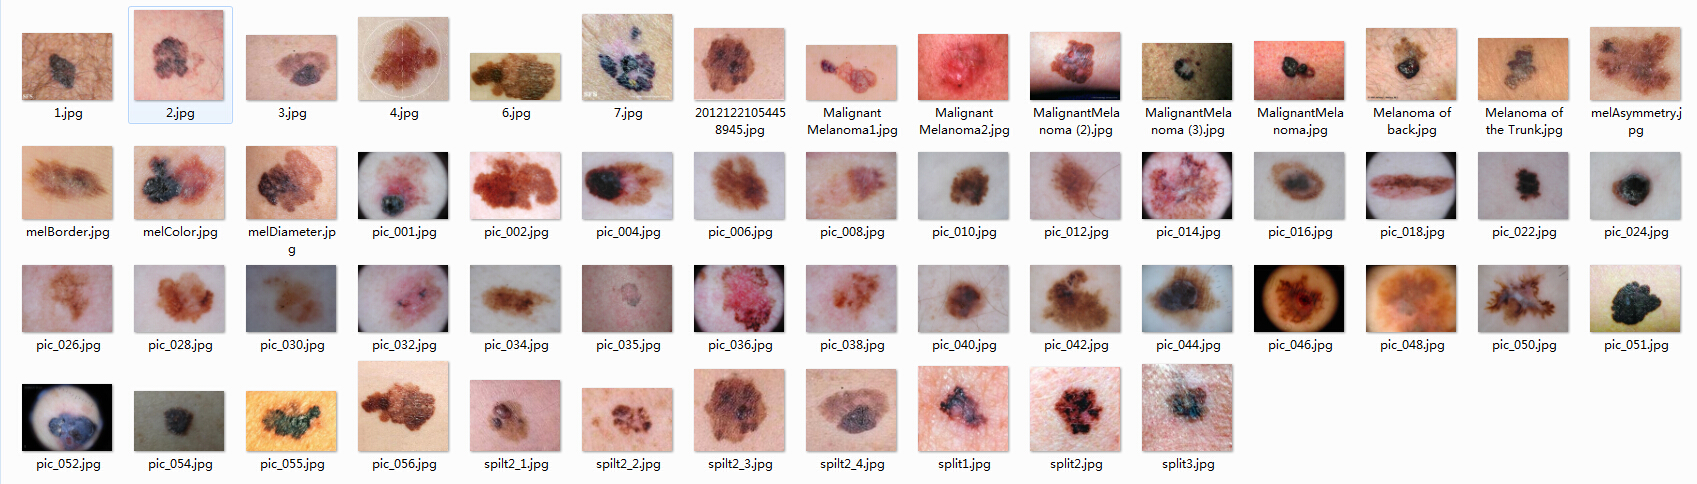
\includegraphics[width=\textwidth]{image/cancers.jpg} 
		\caption{Images of Melanoma class} 
		 \label{fig:ImagesofMelanomaclass} 
	\end{figure}
	\begin{figure}[H]
		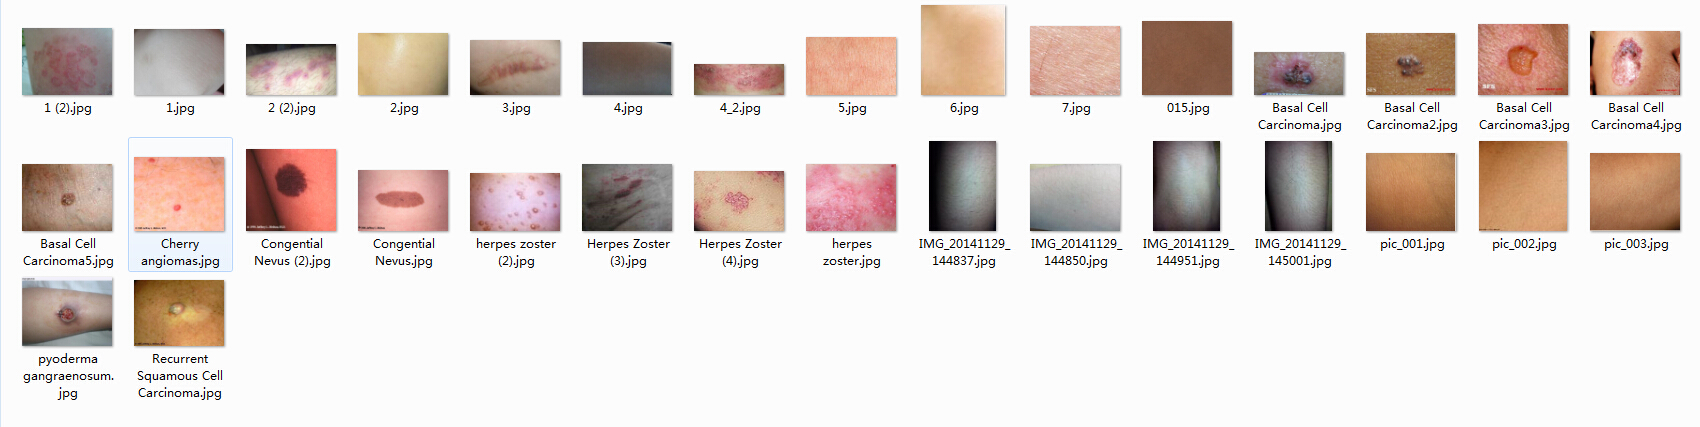
\includegraphics[width=\textwidth]{image/nonecancer.jpg} 
		\caption{Images of none Melanoma class} 
		 \label{fig:ImagesofNoneMelanomaclass} 
	\end{figure}
%	They are located in the \textbf{/dataset/cancer/} and \textbf{/dataset/normal/} directory. 
	There are 56 images in the \textbf{/dataset/cancer/} directory  and 32 in \textbf{/dataset/normal/} directory.
\section{Neural Network}
\subsection{Network definition}
	We use a Neural Network with 13 input , one hidden layer of 50 nodes and an output layer with 2 nodes. 
\subsection{Network input and output}
	We use a 13×1 vector to represent an image's feature, and a 2×1 vector to represent which class this image belongs to.The image feature is the input and the class label is the output.
\subsubsection{Input definition}
	The input feature vector is like below:
	\begin{figure}[H]
		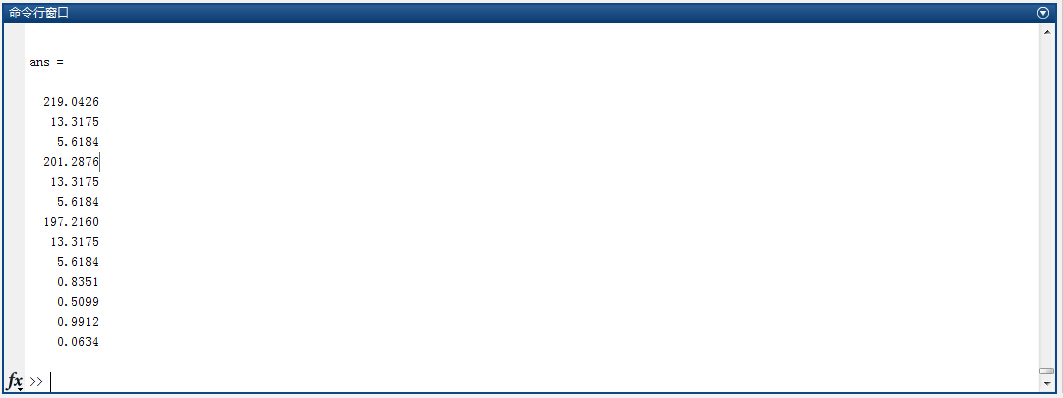
\includegraphics[width=\textwidth]{image/inputfeaturevector.jpg} 
		\caption{Network input vector} 
		 \label{fig:networkInputFeatureVector} 
	\end{figure}
\subsubsection{Output definition}
	For example, when training we will have the 2*1 vector(value of min 0.1 and max 0.9) like this:
	\begin{equation}\label{vec1} \left[ \begin{array}{c} 0.9\\ 0.1\\ \end{array}\right]\end{equation}
	Vector \ref{vec1} means that this image belongs to the first class(the Melanoma class).
	\begin{equation} \label{vec2} \left[ \begin{array}{c} 0.1\\ 0.9\\ \end{array}\right]\end{equation}
	And this above vector \ref{vec2} means that this image belongs to the second class(the none Melanoma class).
\section{Testing}
	\subsection{Changing dataset}
	After adding new images to the dataset directory, you should set in main.m:\\
	\textbf{
	numberofCancer=new number of cancer images;
	\\numberofOther=new number of none cancer images;
	\\reComputeFeature=true;
	\\reTrainNetwork=true;
	}\\Then run the main.m, it may take a long time to recompute all the features.
	\subsection{Using default network}	
	\begin{figure}[H]
		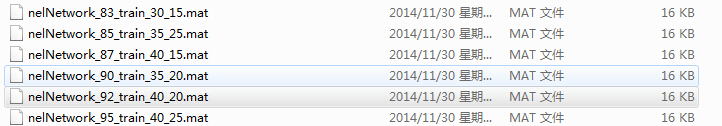
\includegraphics[width=\textwidth]{image/networkSave.jpg} 
		\caption{Networks} 
		 \label{fig:networkSave} 
	\end{figure}
	We have setup some networks like the above picture, user can use them to do the test. 
	\\For example the file: 'nelNetwork\_95\_train\_40\_25.mat' , means that this network's test correct rate is 95\%, and it is trained using the first 40 of 56 cancer images, and also the first 25 of the none cancer images.
	\\If you want to use this network, just change this file's name to 'nelNetwork.mat', and change the parameters in file: trainMyNetwork.m, the trainNumberOfCancer and trainNumberOfOther parameters to those of the network file name. 		\\Like the file nelNetwork\_95\_train\_40\_25.mat, you should set \\
	\textbf{
	trainNumberOfCancer=40 
	\\trainNumberOfOther=25}
	\\ Then inside the main.m, set :\\
	\textbf{
	reComputeFeature=false
	\\reTrainNetwork=false}
	\\Finally, you can run the main.m and get the correct rate.
	\subsection{Train your network}
	Change the parameter trainNumberOfCancer and trainNumberOfOther to what you are going to do experiment on (no larger than the total number of cancer image and none cancer image)inside the trainMyNetwork.m. And set:	\\
	\textbf{
		reComputeFeature=false 
		\\reTrainNetwork=true
	}
	\\in the main.m.
	\subsection{Results}
	\begin{figure}[H]
		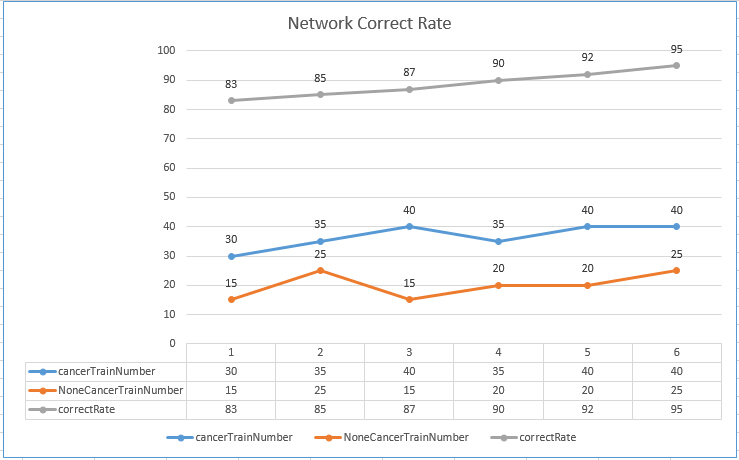
\includegraphics[width=\textwidth]{image/resultTable.jpg} 
		\caption{Network Correct ResultTable} 
		 \label{fig:resultTable} 		 
	\end{figure}
	From the above table, we can know that the more training data we use , the more accurate we get. And the correct rates are all more than 80\%.
\chapter{Future work}
\clearpage
\section{What we can improve:}
\subsection{Data}
	In this case we have totally 80 images to test and train on, and it is a small dataset since it is hard to find many Melanoma images online. So we can get much  improvement if we can get more images to train and to test.
\subsection{Speed}
	It now takes more than 300 seconds to computed all the images' features, and it is quite slow. So maybe we can accelerate by making a better tradeoff between the iteration number of segment algorithm and the correct rate, and make it faster.
\end{document}
